\chapter{Architektur}

\section{Der Hub}
\sectionauthor{\leonard}

Der \emph{Spielehub} ist der zentrale Zugangspunkt, und auch das Erste, was der
Nutzer sieht, wenn er die App startet. Er ist in 3 Teile aufgespalten und
besitzt eine seitliche Navigationsleiste (\emph{Navigation-Drawer}). Jedes Teil
ist dabei ein Fragment. Der Hub besteht aus dem \emph{Spielehub}, welcher die
Spielstände als Liste hält, und den \emph{Kartenspielen} und
\emph{Brettspielen}.


\subsection{Naviagtion Drawer}

Als Menu verwenden wir einen \emph{Navigation-Drawer}, welcher nur im \code{Hub}
zur Verfügung steht und wie folgt aufgebaut ist.

\section{Die Spielstände}
\sectionauthor{\leonard}

Da man Spiele nicht immer in einem Zug durchspielt und man zwischendurch Pause
macht, ist es sinnvoll, das Speichern und Laden der Spiele zu ermöglichen. Für
diese Funktion sind die Klassen \code{SavegameStorage}, \code{Savegame} und
\code{SavegameAdapter} zuständig.

\subsection{Klassen}

\code{Savegame} ist das Spielstand-Objekt, welches alle Daten speichert, die
nötig sind, um ein Spiel fortsetzen zu können. Jedes \code{Savegame} ist dabei
einzigartig.

\code{SavegameStorage} kümmert sich um das Speichern und Laden der
\code{Savegame} Objekte. Diese werden als Liste serialisiert und auf dem Gerät
gespeichert.

\code{SavegameAdapter} erstellt aus den gepeicherten \code{Savegame} Objekten;
für jeden Spielstand eine Karte, welche im Startbildschirm in einer Liste
angezeigt wird. Die Klasse ist etwas komplizierter aufgebaut als die anderen.
Sie besitzt innere Klassen, Vererbungen und eine Interface-Implementierung.

\change{Richter Pfeil (gestrichelt) für Interfaces}
\begin{figure}[h]
	\centering
	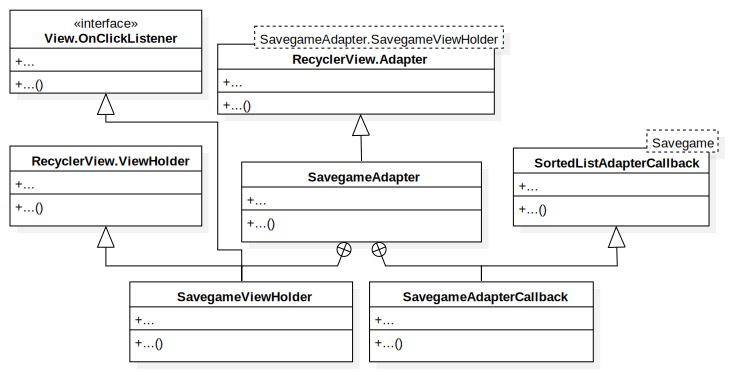
\includegraphics[width=1.0\textwidth]{resources/savegamestorage/SavegameAdapter}
	\caption{Spielstand SavegameAdapter}
\end{figure}

\subsection{Aufbau}
\subsectionauthor{\frank}

Wenn ein Spiel gespeichert oder geladen werden soll, geschieht dies durch einen
Aufruf der Instanz \code{SavegameStorage}. Um hier nicht mehrmals neuen Code,
welche alle Spiele gemeinsam haben, schreiben zu müssen, haben wir diese
Aufgabe an die Klasse \code{GameActivity} abgegeben. Da nun jedes Spiel von
\code{GameActivity} erben soll, müssen dadurch unter anderem zwei abstrakte
Methoden -- zum Speichern und Laden -- implementiert werden.
\code{onSaveGame(Bundle)} respektive \code{onLoadGame(Bundle)}. Diese Methoden
arbeiten jeweils mit einem \textbf{Bundle}, welchem die für einen
Speicherzustand nötigen Informationen übergeben beziehungsweise entnommen
werden können.

Das der Methode \code{onSaveGame} übergebene Bundle kann mit Methoden wie
\code{.putString} oder \code{.putStringArrayList} mit gefüttert werden.
Anschließend werden die gespeicherten Werte weiterverarbeitet und
abgespeichert. Das bedeutet, falls das Bundle unangetastet bleibt, kann
signalisiert werden, dass kein Speichern gewünscht ist, und so der Spielstand
nicht überschrieben wird. Dies ist sehr hilfreich, wenn ein Spiel gestartet,
der Zustand diesen aber nicht verändert wurde. So wird verhindert, dass die
Spielstandliste mit Startaufstellungen von Spielen überfüllt wird. Support für
das Löschen eines Spielstandes ist an dieser Stelle zum aktuellen Zeitpunkt
noch nicht vorhanden.

\change{das in den Anhang}
\begin{figure}[h]
	\centering
	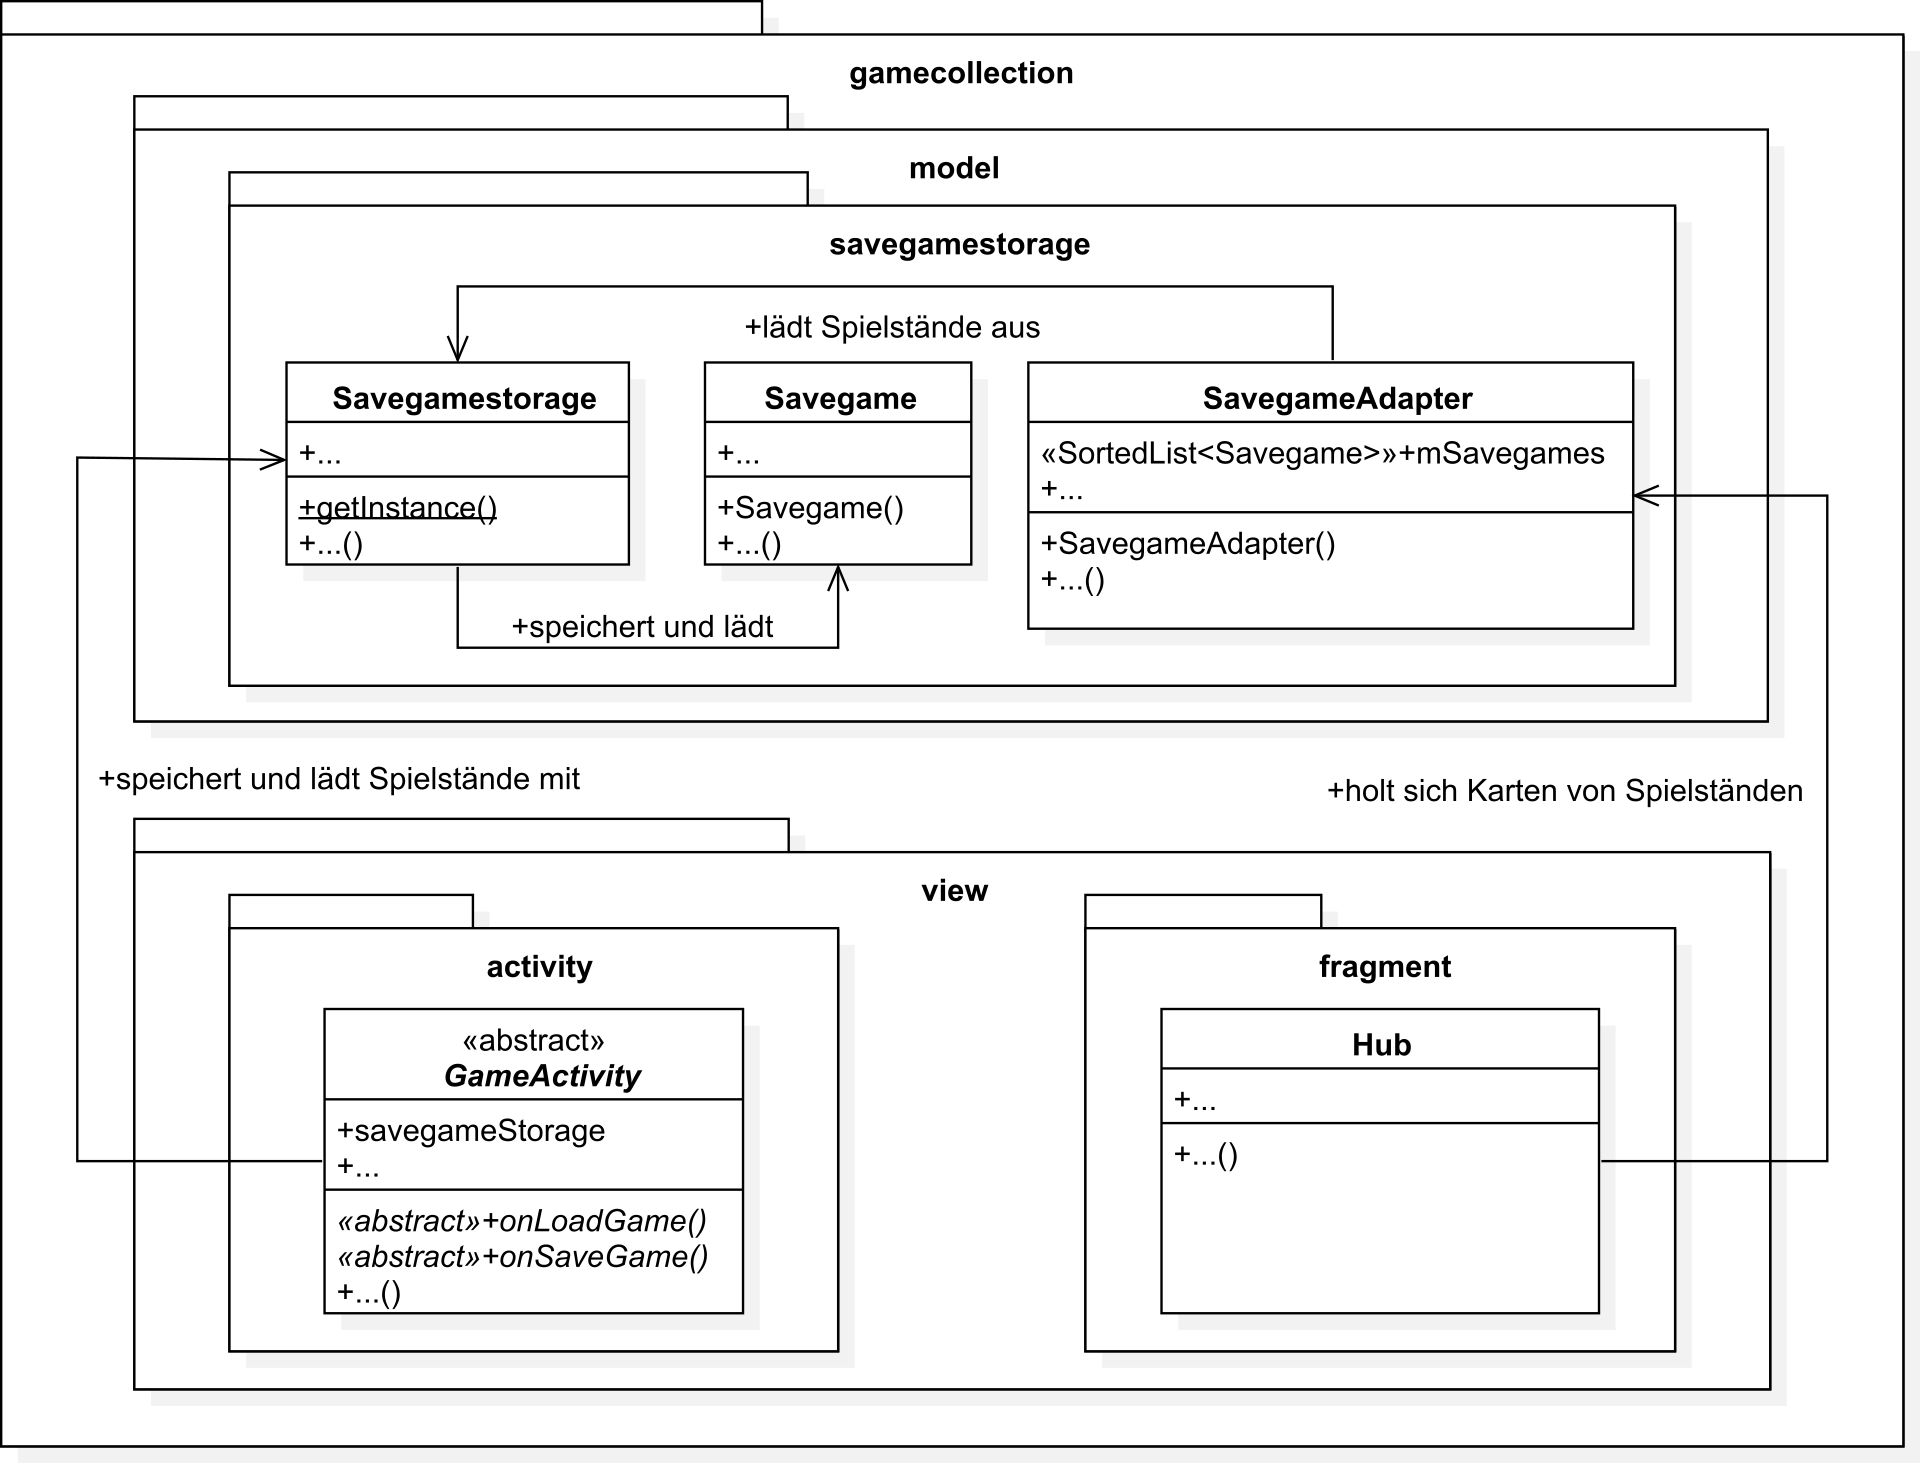
\includegraphics[width=1.0\textwidth]{resources/savegamestorage/Savegamestorage}
	\caption{Spielstand Architektur}
\end{figure}
